\chapter{Configuration interaction}
     A popular post Hartree-Fock method is \textit{configuration interaction}.
     % TODO: Discuss that FCI is "exact" for any choice of basis functions
     It consists of expressing the wavefunction as a linear combination of
     excited Slater determinants in a truncated single-particle and Slater
     determinant basis.
     \begin{align}
         \ket{\Psi}
         &= C\ketslat
         + C^a_i\ketslate{a}{i}
         + \frac{1}{4}C^{ab}_{ij}\ketslate{ab}{ij}
         + \dots,
         \label{eq:ci_wavefunction}
     \end{align}
     where we have divided by a factor $4$ in the double sum to avoid over
     counting as both the coefficients and the excited determinants are
     antisymmetric.
     By generating all the possible Slater determinants from the $L$
     single-particle functions we employ the \textit{full configuration
     interaction} method.
     This will give the most accurate value of the energy for the system, but
     quickly becomes computationally impossible as the FCI space grows in
     dimensions as $\binom{L}{N}$ \cite{kvaal2017notes}.

     A word on notation, we will in the following refrain from using explicit
     excitation indices $a, b, \dots$ and $i, j, \dots$, but rather label the
     coefficients and the Slater determinants by capital letter $I, J, K,
     \dots$.
     That is, we can write \autoref{eq:ci_wavefunction} on the short form
     \begin{align}
         \ket{\Psi}
         &= C_{I}\ket{\Phi_I}.
     \end{align}
     The capital indices will then run over the total number of Slater
     determinants $N_s$ in the full Slater determinant basis.
     This number will depend on the truncation level of the configuration
     interaction wave function.

     \section{Time-independent configuration interaction theory}
        We start with the time-independent Schrödinger equation
        \begin{align}
            \hamil\ket{\Psi_J} = E_J\ket{\Psi_J},
            \label{eq:ci_tise}
        \end{align}
        where $(E_J, \ket{\Psi_J})$ is an eigenpair for $\hat{H}$.
        Expanding the CI wavefunction in a Slater determinant basis.
        \begin{align}
            \ket{\Psi_J} = \sum_{K} C_{KJ}\ket{\Phi_K},
            \label{eq:expanded_ci_wavefunction}
        \end{align}
        where $C_{KJ}$ are the amplitudes for a certain excitation $K$ for a
        specific energy level $J$.
        Inserting \autoref{eq:expanded_ci_wavefunction} into
        \autoref{eq:ci_tise} and left projecting on a state $\ket{\Phi_I}$ we
        get
        \begin{align}
            \sum_{K}\bra{\Phi_I}\hat{H}\ket{\Phi_K}C_{KJ}
            = E_J\sum_{K}\braket{\Phi_I}{\Phi_K}C_{KJ}.
        \end{align}
        We now define the Hamiltonian matrix $H_{IK} =
        \bra{\Phi_I}\hat{H}\ket{\Phi_K}$ and the overlap matrix $S_{IK} =
        \braket{\Phi_I}{\Phi_K}$.
        We can thus formulate the generalized eigenvalue equation
        \begin{gather}
            \sum_{K}H_{IK}C_{KJ} = E_J\sum_{K}S_{IK}C_{KJ}
            \\
            \implies
            HC = ESC,
        \end{gather}
        where $S_{IK} = 1 \iff \braket{\Phi_I}{\Phi_K} = \delta_{IK}$.
        We will in this text only care about systems where the Slater
        determinants are orthonormal.
        Thus the eigenvalue equation we will solve will be
        \begin{align}
            HC = EC,
        \end{align}
        which means our job is to construct $H_{IJ}$ and diagonalize the
        matrix \cite{karwowski}.
        The elements $H_{IJ}$ are computed by
        \begin{align}
            \bra{\Phi_I}\hat{H}\ket{\Phi_J}
            &= \sum_{pq}h^{p}_{q}
            \bra{\Phi_I}\ccr{p}\can{q}\ket{\Phi_J}
            + \frac{1}{4}\sum_{pqrs}u^{pq}_{rs}
            \bra{\Phi_I}\ccr{p}\ccr{q}\can{s}\can{r}\ket{\Phi_J}.
        \end{align}
        Having constructed the one- and two-body elements $h^{p}_{q}$ and
        $u^{pq}_{rs}$ what remains is for us to evaluate the integrals
        $\bra{\Phi_I}\ccr{p}\can{q}\ket{\Phi_J}$ and
        $\bra{\Phi_I}\ccr{p}\ccr{q}\can{s}\can{r}\ket{\Phi_J}$.
        We are then able to construct the configuration interaction matrix
        \begin{align}
            \vfg{\hamilmat}
            &=
            \begin{pmatrix}
                \bra{\Phi_0}\hamil\ket{\Phi_0} &
                \bra{\Phi_0}\hamil\ket{\Phi_1} &
                \dots &
                \bra{\Phi_0}\hamil\ket{\Phi_{N_s}} \\
                \bra{\Phi_1}\hamil\ket{\Phi_0} &
                \bra{\Phi_1}\hamil\ket{\Phi_1} &
                \dots &
                \bra{\Phi_1}\hamil\ket{\Phi_{N_s}} \\
                \vdots & \vdots & \ddots & \vdots \\
                \bra{\Phi_{N_s}}\hamil\ket{\Phi_0} &
                \bra{\Phi_{N_s}}\hamil\ket{\Phi_1} &
                \dots &
                \bra{\Phi_{N_s}}\hamil\ket{\Phi_{N_s}}
            \end{pmatrix}.
        \end{align}
        It is common to see this matrix in block form where we collect
        the different excitation levels in separate blocks.
        For the singles and doubles excitations we get the block matrix
        \begin{align}
            \vfg{\hamilmat}_{\text{CISD}}
            &=
            \begin{pmatrix}
                \bra{\Phi}\hamil\ket{\Phi} &
                \bra{\Phi}\hamil\ket{\Phi^{a}_{i}} &
                \bra{\Phi}\hamil\ket{\Phi^{ab}_{ij}} \\
                \bra{\Phi^{c}_{k}}\hamil\ket{\Phi} &
                \bra{\Phi^{c}_{k}}\hamil\ket{\Phi^{a}_{i}} &
                \bra{\Phi^{c}_{k}}\hamil\ket{\Phi^{ab}_{ij}} \\
                \bra{\Phi^{cd}_{kl}}\hamil\ket{\Phi} &
                \bra{\Phi^{cd}_{kl}}\hamil\ket{\Phi^{a}_{i}} &
                \bra{\Phi^{cd}_{kl}}\hamil\ket{\Phi^{ab}_{ij}} \\
            \end{pmatrix}.
        \end{align}

        \subsection{Truncated configuration interaction}
            % TODO: Demonstrate truncated configuration interaction and discuss
            % its disadvantages such as lack of size extensivity and size
            % consistency.
            As an example of <size extensivity/size consitency> we demonstrate
            the troubles arising when we restrict ourselves to a system of two
            particles and four basis functions.
            Our basis thus consists of the spin-orbitals $\brac{\ket{\phi_1},
            \ket{\phi_2}, \ket{\phi_3}, \ket{\phi_4}}$, with the reference
            Slater determinant
            \begin{align}
                \ket{\Phi}
                &= \frac{1}{\sqrt{2}}\brac{
                    \ket{\phi_1\phi_2}
                    - \ket{\phi_2\phi_1}
                }.
                % TODO: It might not be necessary to show what the determinant
                % looks like.
            \end{align}
            Using truncated configuration interaction with singles excitations
            only, we get the many-body wave function
            \begin{align}
                \ket{\Psi}
                &= C\ket{\Phi}
                + C^{a}_{i}\ket{\Phi^{a}_{i}}
                = C\ket{\Phi}
                + C^{3}_{1}\ket{\Phi^{3}_{1}}
                + C^{4}_{1}\ket{\Phi^{4}_{1}}
                + C^{3}_{2}\ket{\Phi^{3}_{2}}
                + C^{4}_{2}\ket{\Phi^{4}_{2}}.
                \label{eq:cis_wave_function}
            \end{align}
            Graphically we can represent the full space of the Slater determinants
            by \autoref{fig:tiny-slater-basis}.
            Comparing with \autoref{eq:cis_wave_function} we see that the only
            determinant missing in the truncated wave function is the doubly
            excited determinant $\ket{\Phi^{34}_{12}}$.
            Stated a little differently, truncated configuration interaction is
            not able to exploit the full space of Slater determinants.
            The method also fails in ``removing all trace`` of the reference
            state.
            This means that truncated configuration interaction will not be able
            to fully excite the reference state.
            Note that the example shown in \autoref{eq:cis_wave_function} and
            \autoref{fig:tiny-slater-basis} extends for more particles and
            higher truncation levels for configuration interaction.
            For example for a system with four particles and truncated
            configuration interaction with singles and doubles excitations this
            same behaviour is exhibited.
            % TODO: Explain how this problem becomes worse for more basis
            % functions.
            % TODO: Explain how coupled cluster fixes this problem in the
            % chapter on coupled cluster.
            \begin{figure}
                \begin{center}
                    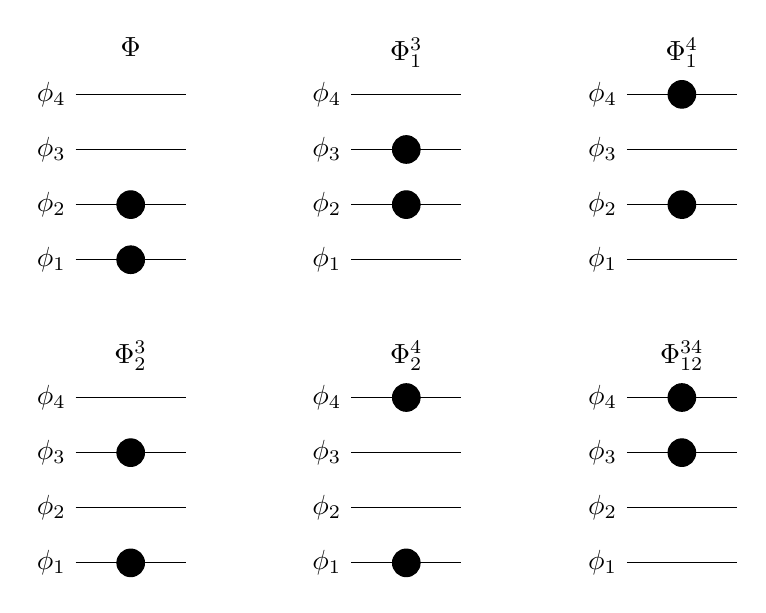
\begin{tikzpicture}[scale=0.7]
                        % State 1
                        \begin{scope}
                            \foreach \i in {1,...,4} {
                                \draw (-1, \i - 1) node[anchor=east]
                                {$\ket{\phi_{\i}}$} -- (1, \i - 1);
                            }
                            \filldraw (0,4.2) node[anchor=north]
                                {$\ket{\Phi}$};
                            \filldraw (0, 0) circle (0.25cm);
                            \filldraw (0, 1) circle (0.25cm);
                        \end{scope}

                        % State 2
                        \begin{scope}[xshift=5cm]
                            \foreach \i in {1,...,4} {
                                \draw (-1, \i - 1) node[anchor=east]
                                {$\ket{\phi_{\i}}$} -- (1, \i - 1);
                            }
                            \filldraw (0,4.2) node[anchor=north]
                                {$\ket{\Phi^{3}_{1}}$};
                            \filldraw (0, 2) circle (0.25cm);
                            \filldraw (0, 1) circle (0.25cm);
                        \end{scope}

                        % State 3
                        \begin{scope}[xshift=10cm]
                            \foreach \i in {1,...,4} {
                                \draw (-1, \i - 1) node[anchor=east]
                                {$\ket{\phi_{\i}}$} -- (1, \i - 1);
                            }
                            \filldraw (0,4.2) node[anchor=north]
                                {$\ket{\Phi^{4}_{1}}$};
                            \filldraw (0, 3) circle (0.25cm);
                            \filldraw (0, 1) circle (0.25cm);
                        \end{scope}

                        % State 4
                        \begin{scope}[yshift=-5.5cm]
                            \foreach \i in {1,...,4} {
                                \draw (-1, \i - 1) node[anchor=east]
                                {$\ket{\phi_{\i}}$} -- (1, \i - 1);
                            }
                            \filldraw (0,4.2) node[anchor=north]
                                {$\ket{\Phi^{3}_{2}}$};
                            \filldraw (0, 0) circle (0.25cm);
                            \filldraw (0, 2) circle (0.25cm);
                        \end{scope}

                        % State 5
                        \begin{scope}[yshift=-5.5cm, xshift=5cm]
                            \foreach \i in {1,...,4} {
                                \draw (-1, \i - 1) node[anchor=east]
                                {$\ket{\phi_{\i}}$} -- (1, \i - 1);
                            }
                            \filldraw (0,4.2) node[anchor=north]
                                {$\ket{\Phi^{4}_{2}}$};
                            \filldraw (0, 0) circle (0.25cm);
                            \filldraw (0, 3) circle (0.25cm);
                        \end{scope}

                        % State 6
                        \begin{scope}[yshift=-5.5cm, xshift=10cm]
                            \foreach \i in {1,...,4} {
                                \draw (-1, \i - 1) node[anchor=east]
                                {$\ket{\phi_{\i}}$} -- (1, \i - 1);
                            }
                            \filldraw (0,4.2) node[anchor=north]
                                {$\ket{\Phi^{34}_{12}}$};
                            \filldraw (0, 3) circle (0.25cm);
                            \filldraw (0, 2) circle (0.25cm);
                        \end{scope}
                    \end{tikzpicture}
                \end{center}
                \caption{In this figure we can see the six possible Slater
                determinants, i.e., all the basis Slater determinants, made from
                the four basis functions $\brac{\ket{\phi_1}, \ket{\phi_2},
                \ket{\phi_3}, \ket{\phi_4}}$ with two particles.}
                \label{fig:tiny-slater-basis}
            \end{figure}

        \subsection{Constructing the Slater determinants}
            % TODO: Explain how to construct bit strings representing
            % determinants.

        \subsection{Evaluating the matrix elements}
            As the one- and two-body elements $\oneten^{p}_{q}$ and
            $\twoten^{pq}_{rs}$ are known in advance, our task is to evaluate
            the overlap between Slater determinants acted upon by creation and
            annihilation operators.

        \subsection{The Slater-Condon rules}

        \subsection{Brillouin's theorem}
            % TODO: Consider moving this subsection to the chapter on
            % Hartree-Fock
            Brillouin's theorem states that given an orthonormal single-particle
            basis $\brac{\ket{\phi_p}}_{i = 1}^{L}$, which is used to build a basis of
            Slater determinants $\brac{\ket{\Phi_I}}_{I = 1}^{N_s}$, then
            \begin{align}
                \bra{\Phi}\hamil\ket{\Phi^{a}_{i}} = 0,
            \end{align}
            is true iff the single-particle basis is found from solving the
            Hartree-Fock equations and $\ket{\Phi^{a}_{i}}$ is any singly
            excited determinant from the reference determinant $\ket{\Phi}$
            \cite{kvaal2017notes}.
            An important consequence of this is that all single excitations,
            from the reference state, can be neglected if we choose the
            Hartree-Fock reference state as our reference determinant.
            \begin{proof}
                We prove Brillouin's theorem directly by evaluating the matrix
                element
                \begin{align}
                    \bra{\Phi}\hamil\ket{\Phi^{a}_{i}}
                    &= \bra{\Phi}\onehamil\ket{\Phi^{a}_{i}}
                    + \frac{1}{4}\bra{\Phi}\twohamil\ket{\Phi^{a}_{i}}
                    = h^{a}_{i} + u^{aj}_{ij}
                    = f^{a}_{i} = 0,
                \end{align}
                when the single-particle basis is the molecular orbitals found
                from solving the Hartree-Fock equations
                \begin{align}
                    \fock\ket{\phi_p} = \varepsilon_p\ket{\phi_p},
                \end{align}
                making the Fock matrix diagonal.
            \end{proof}

        \subsection{One-body density matrix}
            For a given eigenstate $\ket{\Psi_I}$ of the many-body Hamiltonian
            shown in \autoref{eq:ci_tise} we can compute the one-body density
            matrix ${\rho_I}^{q}_{p}$ by
            \begin{align}
                {\rho_I}^{q}_{p}
                &= \bra{\Psi_I}\ccr{p}\can{q}\ket{\Psi_I}
                = C_{JI}^{*}C_{KI}\bra{\Phi_J}\ccr{p}\can{q}\ket{\Phi_K}.
            \end{align}

    \section{Time-dependent configuration interaction}
        Starting from the time-depdendent Schrödinger equation, we can formulate
        the time-evolution of the many-body wave function.
        \begin{align}
            i\hslash \dpd[]{}{t}\ket{\Psi(t)}
            = \hamil(t)\ket{\Psi(t)},
            \label{eq:ci_tdse}
        \end{align}
        Here the time-dependent wave function $\ket{\Psi(t)}$ is given as a
        linear combination of Slater determinants
        \begin{align}
            \ket{\Psi(t)} = c_{I}(t) \ket{\Phi_I},
            \label{eq:ci_td_wave}
        \end{align}
        where the orbitals in the Slater determinants are static, i.e.,
        time-independent, meaning that the time-evolution happens in the
        coefficients $c_{I}(t)$.
        Our choice of initial state $\ket{\Psi(0)}$ is to a large degree
        arbitrary as long as the coefficients are normalized and the
        determinants span the entire space we are looking at.
        A natural choice is to choose $\ket{\Psi(0)} = \ket{\Psi_J}$, where
        $\ket{\Psi_J}$ is an eigenstate from the time-independent Schrödinger
        equation in \autoref{eq:ci_tise}.
        It is common to choose $J = 0$, i.e., the ground state, but there is
        nothing stopping us from choosing an arbitrary initial guess.
        For example, we can choose a single Slater determinant from our basis of
        determinants as an initial guess.
        This can be a good guess, especially if we use Hartree-Fock orbitals as
        our basis of spin-orbitals.

        Inserting \autoref{eq:ci_td_wave} into \autoref{eq:ci_tdse} we get an
        equation for time-evolution of the coefficients.
        \begin{align}
            i\hslash \dpd[]{}{t}c_{J}(t)\ket{\Phi_J}
            = \hamil(t) c_{J}(t)\ket{\Phi_J}.
        \end{align}
        Left-projecting with a Slater determinant $\ket{\Phi_I}$ then yields
        \begin{gather}
            i\hslash \dpd[]{}{t}c_{J}(t)\braket{\Phi_I}{\Phi_J}
            = \bra{\Phi_I}\hamil(t)\ket{\Phi_J} C_{J}(t) \\
            \implies
            i\hslash \dpd[]{}{t}c_{J}(t) S_{IJ}
            = H_{IJ}(t) c_{J}(t),
        \end{gather}
        where we've again introduced the matrix $S_{IJ}$ with overlaps between
        the Slater determinants and the time-dependent Hamiltonian matrix
        $H_{IJ}(t)$.
        We'll limit our attention to systems where the Slater determinants are
        orthonormal, thus leaving us with the equation
        \begin{align}
            i\hslash \dpd[]{}{t}c_{I}(t)
            = H_{IJ}(t) c_{J}(t).
            \label{eq:tdci}
        \end{align}
        As the initial coefficients $c_{I}(0)$ are known, we need to compute the
        matrix elements of the time-dependent Hamiltonian at each time step
        before using a time-evolution scheme to solve \autoref{eq:tdci}.
        Depending on the nature of the time-dependent interaction in the
        Hamiltonian, we can compute the time-dependent matrix elements by
        \begin{align}
            H_{IJ}(t)
            &= \bra{\Phi_I}\hamil(t)\ket{\Phi_J}
            = \bra{\Phi_I}\onehamil(t)\ket{\Phi_J}
            + \frac{1}{4}\bra{\Phi_I}\twohamil(t)\ket{\Phi_J}
            \\
            &=
            \oneten^{p}_{q}(t)
            \bra{\Phi_I}\ccr{p}\can{q}\ket{\Phi_J}
            + \frac{1}{4}\twoten^{pq}_{rs}(t)
            \bra{\Phi_I}\ccr{p}\ccr{q}\can{s}\can{r}\ket{\Phi_J}.
        \end{align}
